\subsection{Initial-model full-DD resolution and shared-pick noise}

A separate calculation now includes both absolute picks and catalog
differences in the local resolution operator. It is evaluated at the saved
initial sources and velocity model, with stage-0 weights, rather than at a
converged tomography result. The identified subset contains 1,092 events,
14,262 primitive picks and 44,718 catalog differences. Of the 58,980
observations, 58,671 have active weighted rows. The linear system retains
4,368 source parameters and 462 velocity nodes, with the exported DD mask,
1,201 smoothing rows and column-scaled damping. No waveform difference enters
this calculation.

Let $A$ be the weighted, masked data matrix and let
$H=A^{\mathsf T}A+L^{\mathsf T}L+D^{\mathsf T}D$, where $L$ and $D$ are the
exported smoothing and damping operators. The model resolution is the
velocity-model block of $H^{-1}A^{\mathsf T}A$. Source elimination retains
the coupling to location and origin-time increments. For the primitive pick
errors, the incidence matrix $P$ places the same pick error in each absolute
observation and in every catalog difference that contains it. With fixed row
weights $W$ and assumed pick covariance $\Sigma_p$, define
\begin{equation}
 K_q=\left(H^{-1}A^{\mathsf T}W P\Sigma_p^{1/2}\right)_q,
 \qquad C_q=K_qK_q^{\mathsf T}.
\end{equation}
Here $q$ denotes the log-slowness model parameters. This propagated picking
noise is not the inverse-normal posterior covariance. Reported symmetric
pick uncertainties are treated as one standard deviation, although their
provider confidence levels are unavailable. This is an assumption about
timing uncertainty, unrelated to waveform instrument-response corrections.

The numerical calculation completed with a model Schur condition number of
$2.30\times10^3$. Relative residuals of the source, resolution and noise
transfer equations are $6.53\times10^{-16}$, $5.95\times10^{-16}$ and
$1.05\times10^{-15}$, respectively. These residuals test the linear algebra.
The separate input review checked all 14,262 native rays, their saved geometry
and the corresponding source-matrix entries. Initial-model comparison against
the existing layered reference gives maximum time and source-vector
differences of $9.59\times10^{-7}$ s and $1.78\times10^{-6}$ s/km. These
checks do not establish accuracy after a three-dimensional model update.

Figure~\ref{fig:initialfulldd} shows the resulting sections.
The nodal masked-resolution diagonal ranges from
$-1.65\times10^{-5}$ to $0.802$. Small negative values remain in the saved
results and display; they are not clipped to zero. The nodal picking-noise
standard deviation ranges from $0.00405$ to $0.0494$ km/s. At a displayed
point with trilinear weights $w$, the velocity variance is
\begin{equation}
 \sigma_v^2=w C_v w^{\mathsf T},\qquad
 C_v=\operatorname{diag}(v)C_q\operatorname{diag}(v).
\end{equation}
Thus the display propagates the full covariance to interpolated velocity.
The resolution column instead interpolates the saved nodal diagonal for
display; it does not define a pointwise resolution operator.

All quantities remain conditional on the initial model, fixed weights,
computed ray branches, masks, smoothing and damping. Active source bounds,
nonlinear changes, model and ray errors, correlated station errors,
regularization bias and selection effects are outside this covariance.
This closes the initial-model full-DD calculation but does not replace the
missing final-model resolution or reproduce the manuscript's Figure 11.
The authoritative subset and its differences from the study remain explicit.
The saved matrices, node and pick tables, full identifier companions and
replay commands are preserved in
\path{data/development/hayward_initial_full_dd_resolution_001/}.
A fresh replay from the packaged inputs reproduced both CSV tables, the
matrix archive and both identifier companions byte for byte. All four
numerical arrays matched exactly; only the input paths in the new numerical
manifest changed. A separate portable replot reproduced the section table,
PDF and PNG exactly. These replays test the two documented procedures; they
do not rerun the ray export or complete the nonlinear inversion workflow.

\begin{figure}[p]
\centering
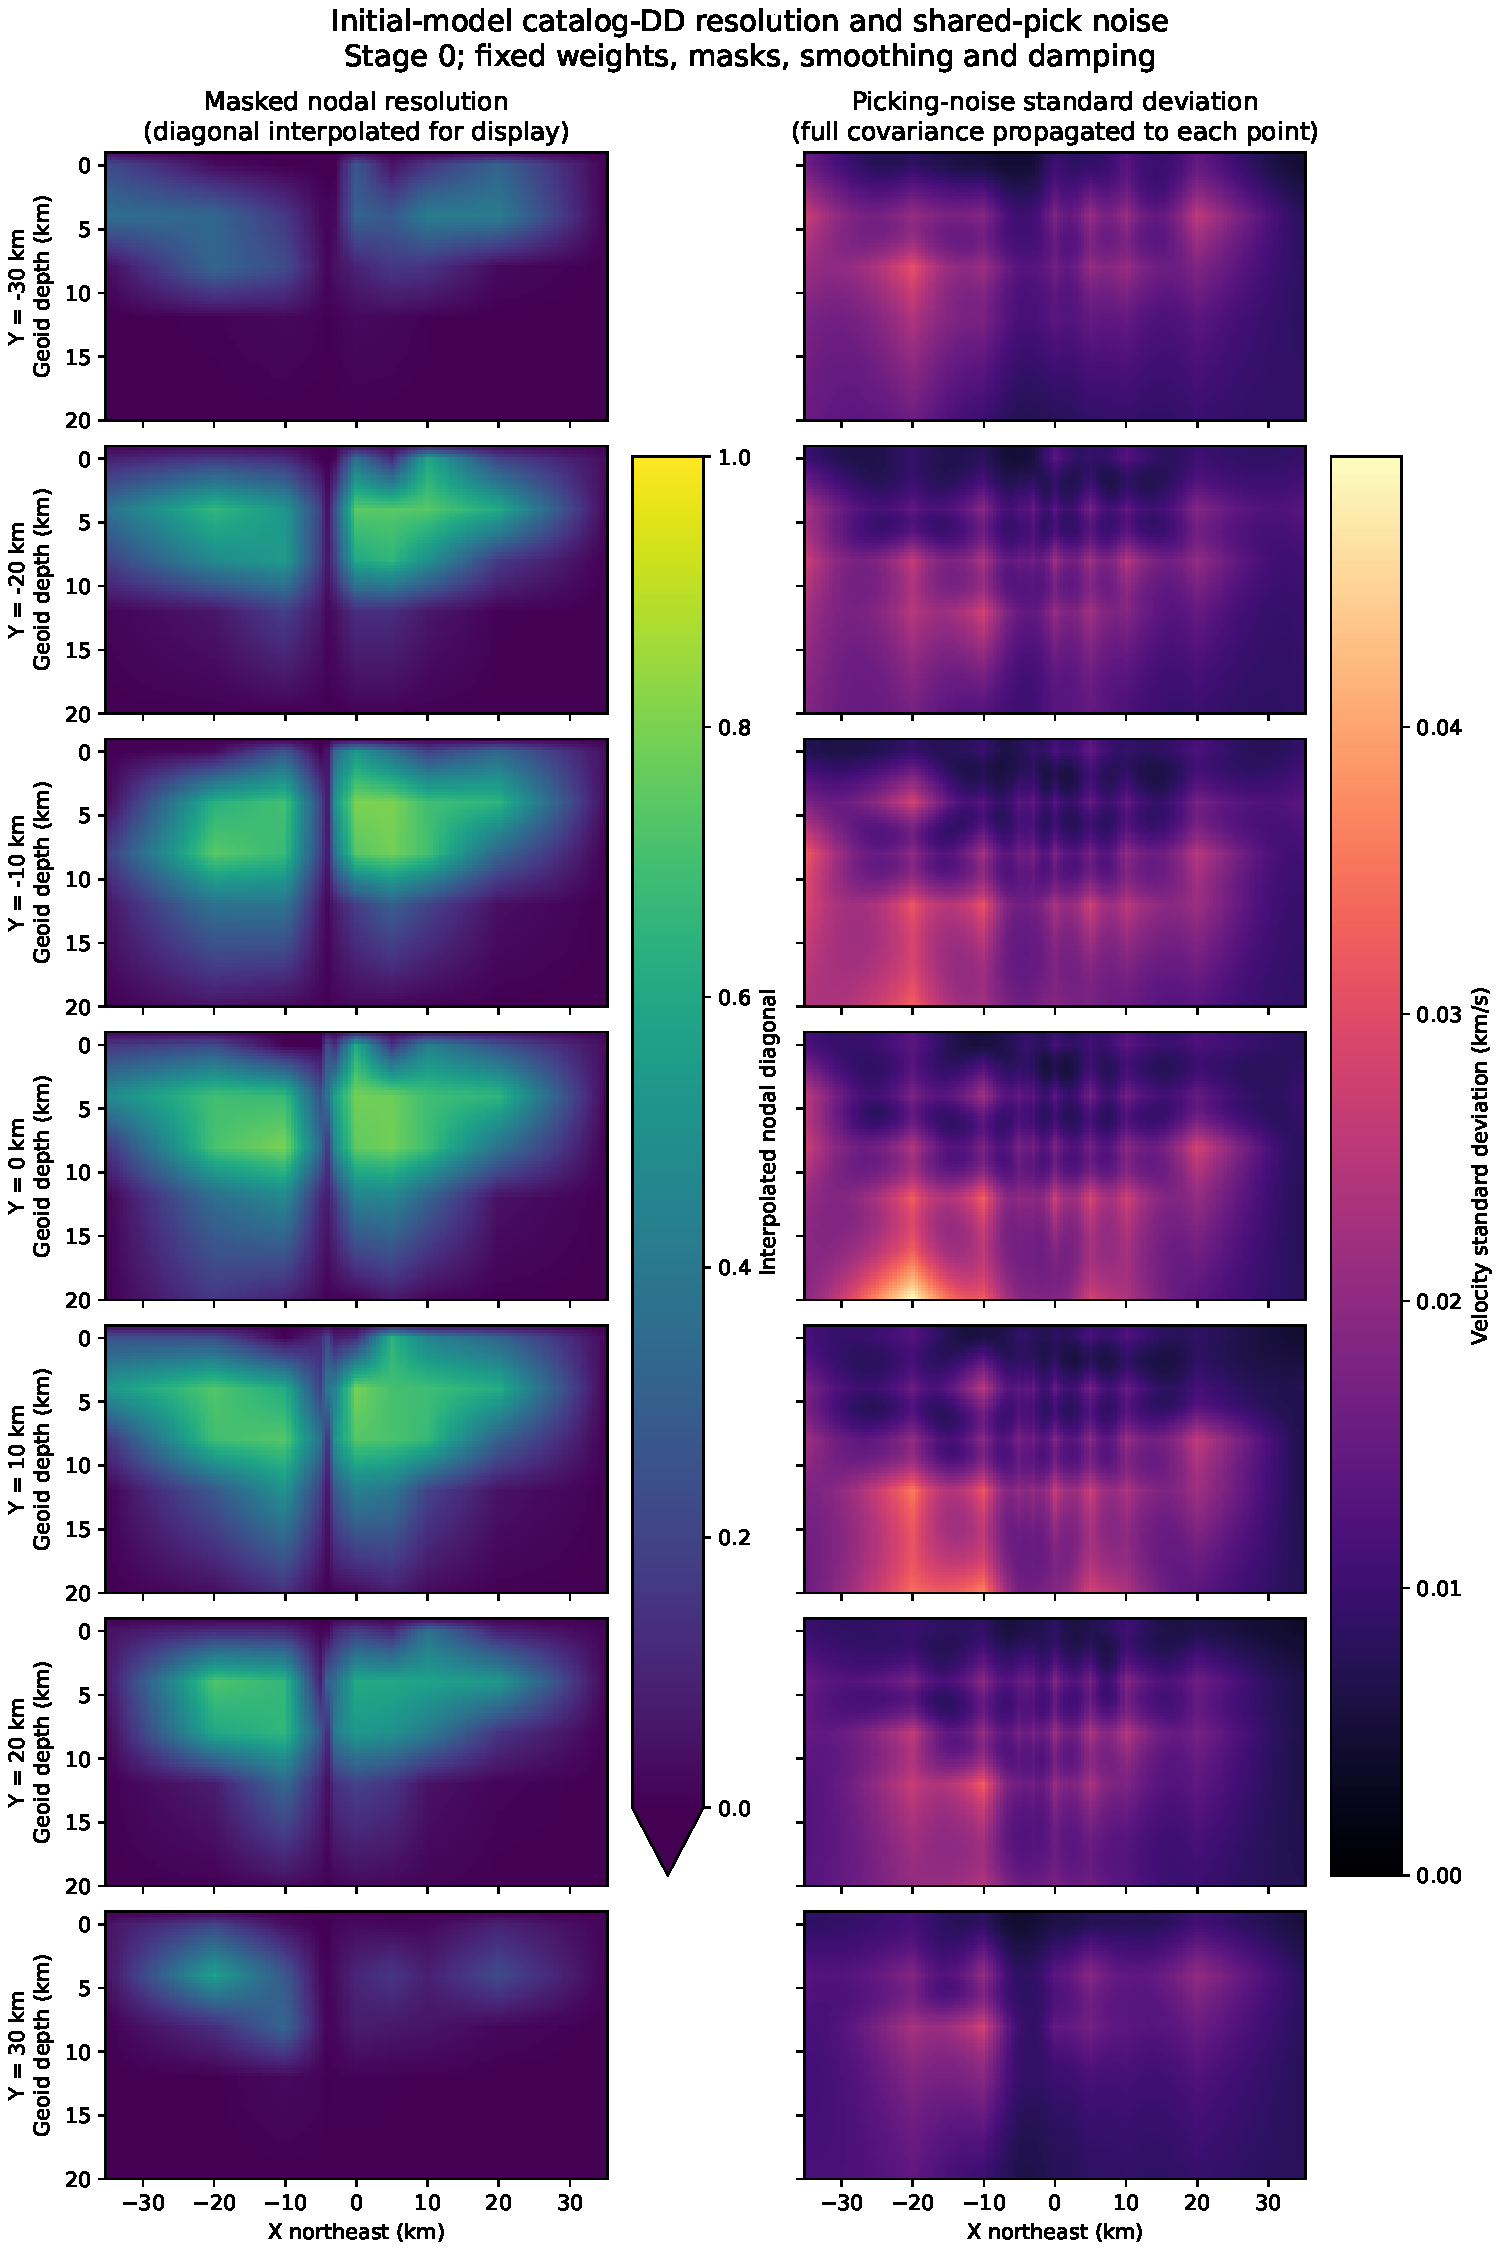
\includegraphics[width=\linewidth,height=0.82\textheight,keepaspectratio]{../data/development/hayward_initial_full_dd_resolution_001/figure/initial_full_dd_resolution.pdf}
\caption{Initial-model catalog-DD resolution and conditional picking noise.
Rows show seven cross-fault sections in the documented local coordinates.
Left: the masked nodal-resolution diagonal, interpolated for display; the
lower colorbar extension retains its small negative values. Right: velocity
standard deviation after propagating the full shared-pick covariance through
the trilinear basis. All sections use the same scales. The calculation fixes
the initial sources, velocity, stage-0 weights, masks and regularization.
It is neither final-model uncertainty nor a reproduced Figure 11.}
\label{fig:initialfulldd}
\end{figure}
